\documentclass[submit]{harvardml}

\course{CS181-S20}
\assignment{Assignment \#5}
\duedate{7:59pm EST, April 2, 2021}

\newcommand{\attr}[1]{\textsf{#1}}
\usepackage[OT1]{fontenc}
\usepackage[colorlinks,citecolor=blue,urlcolor=blue]{hyperref}
\usepackage[pdftex]{graphicx}
\usepackage{subfig}
\usepackage{framed}
\usepackage{fullpage}
\usepackage{amsmath}
\usepackage{amssymb}
\usepackage{color}
\usepackage{todonotes}
\usepackage{listings}
\usepackage{common}
\usepackage{bm}
\usepackage{enumitem}
\usepackage{tikz}
\usetikzlibrary{positioning,shapes,arrows}
\usepackage{xifthen}
\usepackage{soul}

\usepackage[mmddyyyy,hhmmss]{datetime}

\definecolor{verbgray}{gray}{0.9}

\lstnewenvironment{csv}{
  \lstset{backgroundcolor=\color{verbgray},
  frame=single,
  framerule=0pt,
  basicstyle=\ttfamily,
  columns=fullflexible}}{}

\begin{document}


\begin{center}
{\Large Homework 5: EM with Mixtures, PCA, and Graphical Models}\\
\end{center}

This homework assignment will have you work with EM for mixtures, PCA,
and graphical models. We encourage you to read sections 9.4 and 8.2.5 of the course textbook.

Please type your solutions after the corresponding problems using this
\LaTeX\ template, and start each problem on a new page.

Please submit the \textbf{writeup PDF to the Gradescope assignment `HW5'}. Remember to assign pages for each question.

Please submit your \textbf{\LaTeX\ file and code files to the Gradescope assignment `HW5 - Supplemental'}. 


\begin{problem}[Expectation-Maximization for Categorical-Geometric Mixture Models, 25pts]

In this problem we will explore expectation-maximization for a
Categorical-Geometric Mixture model.

Specifically, we assume that there are a set of $K$ parameters $p_k
\in [0,1]$.  To generate each observation $n$, we first choose which
of those $K$ parameters we will use based on the (unknown) overall
mixing proportion over the components $\btheta \in [0,1]^K$,
where~${\sum_{k=1}^K \theta_k=1}$.  Let the (latent) $\boldz_n$ indicate
which of the $K$ components we use to generate observation $n$.  Next
we sample the observation $x_n$ from a geometric distribution
with parameter $p_{\boldz_n}$.  This process can be written as: 
\begin{eqnarray*}
 \boldz_n &\sim& \text{Categorical}(\btheta) \\
 x_n &\sim& \text{Geometric}(p_{\boldz_n} )
\end{eqnarray*}
We encode observation $n$'s latent
component-assignment ${\boldz_n \in
  \{0,1\}^K}$ as a one-hot vector. Element indicator variables $z_{n k}$ equal 1 if $\boldz_n$ was generated using component $k$.

A geometric distribution corresponds to the number of trials
needed to get to the first success. If success occurs with probability
$p$, its PMF is given by $p(x_n ; p_k) = (1 - p_k)^{x_n - 1} p_k$, where $x_n \in \{1, 2, ...\}$.

  \begin{enumerate}

  \item \textbf{Intractability of the Data Likelihood} We are
    generally interested in finding a set of parameters $p_k$ that
    maximize the data likelihood $\log
    p(\{x_n\}^N_{n=1}; \btheta, \{p_k\}^K_{k = 1})$.  Expand the data
    likelihood to include the necessary sums over observations
    $x_n$ and to marginalize out (via more sums) the latents
    $\boldz_n$.  Why is optimizing this likelihood directly
    intractable?  

\item \textbf{Complete-Data Log Likelihood} The complete data
  $D = \{(x_n, \boldz_n)\}_{n=1}^N$ includes latents $\boldz_n$. Write
  out the complete-data negative log likelihood. Apply the ``power trick''\footnote{The ``power trick'' is used when terms in a PDF are raised to the power of indicator components of a one-hot vector.  For example, it allows us to rewrite $p(\boldz_n ;  \btheta) = \prod_k \theta_k^{z_{nk}}$.} and simplify your expression using indicator elements $z_{n k}$.

\[\mcL(\btheta, \{p_k\}^K_{k=1}) =  -\ln p(D; \btheta, \{p_k\}^K_{k=1}).\]

Note that optimizing
  this loss is now computationally tractable if we know $\boldz_n$.

\item \textbf{Expectation Step} Our next step is to introduce a
  mathematical expression for $\boldq_n$, the posterior over the
  hidden topic variables~$\boldz_n$ conditioned on the observed data
  $x_n$ with fixed parameters, i.e $\boldq_n = p(\boldz_n | x_n;
  \btheta, \{ p_k \}^K_{k=1})$.

\begin{itemize}
\item  \textbf{Part 3.A } Write down and simplify the expression for $\boldq_n$.  Note that because the $\boldq_n$ represents the posterior over the hidden categorical variables $\boldz_n$, the components of vector $\boldq_n$ must sum to 1.

\item  \textbf{Part 3.B } Give an algorithm for calculating the expression for $\boldq_n$ found in Part 3.A for all $n$, given the observed data~$\{x_n\}^N_{n=1}$ and settings of the parameters~$\btheta$ and~$\{ p_k\}^K_{k=1}$.

\end{itemize}

\item \textbf{Maximization Step}
Using the~$\boldq_n$ estimates from the Expectation Step, derive an update for maximizing the expected complete data log likelihood in terms of~$\btheta$ and~$\{ p_k \}^K_{k=1}$.

\begin{itemize}
    \item \textbf{Part 4.A } Derive an expression for the expected complete-data log likelihood using $\boldq_n$.
    \item \textbf{Part 4.B } Find an expression for $\btheta$ that maximizes this expected complete-data log likelihood. You may find it helpful to use Lagrange multipliers in order to enforce the constraint $\sum \theta_k = 1$. Why does this optimal $\btheta$ make intuitive sense?
    \item \textbf{Part 4.C } Find an expression for the $\{p_k \}^K_{k = 1}$ that maximize the expected
      complete-data log likelihood.  Why does this optimal $\{p_k \}^K_{k = 1}$  make intuitive sense?
\end{itemize}

\item Suppose that this had been a classification problem. That is,
  you were provided the ``true'' categories $\boldz_n$ for each observation $x_n$,
  and you were going to perform the classification by
  inverting the provided generative model (i.e. now you're predicting $z$ given $x$). Could you reuse any of
  your inference derivations above?
  
  (Continued on next page.)
  \end{enumerate}
  
  



\end{problem}

\newpage

\begin{framed}
\noindent\textbf{Problem 1} (cont.)\\
\begin{enumerate}

\item[6.] Finally, implement your solution (see \texttt{T5\_P1.py} for starter code).  You are responsible for implementing the \texttt{expected\_loglikelihood}, \texttt{e\_step} and \texttt{m\_step} functions. Test it out with data given
  $10$ samples from $3$ components with $p_1 = .1$, $p_2=.5$, and
  $p_3=.9$.  How does it perform?  What if you increase the number of
  samples to $1000$ from each of the components?  What if you change
  $p_2=.2$?  Hypothesize reasons for the differences in performance
  when you make these changes. You may need to record five to ten trials (random restarts) in order to observe meaningful insights.
\end{enumerate}
  
\end{framed}  

\subsection*{Solution}

\newpage

\begin{problem}[PCA, 15 pts]

For this problem you will implement PCA from scratch.  Using
\texttt{numpy} to call SVDs is fine, but don't use a third-party
machine learning implementation like \texttt{scikit-learn}.

We return to the MNIST data set from T4. You have been given
representations of 6000 MNIST images, each of which are $28\times28$
greyscale handwritten digits. Your job is to apply PCA on MNIST, and
discuss what kind of structure is found.

The given code in \texttt{T5\_P2.py} loads the images into your environment.  File \texttt{T5\_P2\_Autograder.py} contains a test case to check your cumulative proportion of variance.

\begin{enumerate}

\item Compute the PCA. Plot the eigenvalues corresponding to the most significant 500
  components in order from most significant to least. Make another plot that describes the cumulative proportion of variance explained by the first $k$ most significant components for values of $k$ from 1 through 500.
  How much variance is explained by the first 500 components?  Describe
  how the cumulative proportion of variance explained changes with $k$.

\item Plot the mean image of the dataset and plot an image corresponding to each of the
  first 10 principle components.  How do the principle component images compare to the
  cluster centers from K-means? Discuss any similarities and
  differences.  Include all 11 plots in your PDF submission.

\item Compute the reconstruction error on the data set using the mean
  image of the dataset. Then compute the reconstruction error using the first 10 principal components. How do these
  errors compare to the final objective loss achieved by using K-means on the dataset? Discuss any similarities and
  differences.

\end{enumerate}


\textit{Include your plots in your PDF. There may be several plots for this problem, so feel free
to take up multiple pages.}






\end{problem}


\subsection*{Solution}

\newpage

\begin{problem}[Bayesian Networks, 10 pts]

  \noindent In this problem we explore the conditional independence
  properties of a Bayesian Network.  Consider the following Bayesian
  network representing a fictitious person's activities. Each random
  variable is binary (true/false).

\begin{center}
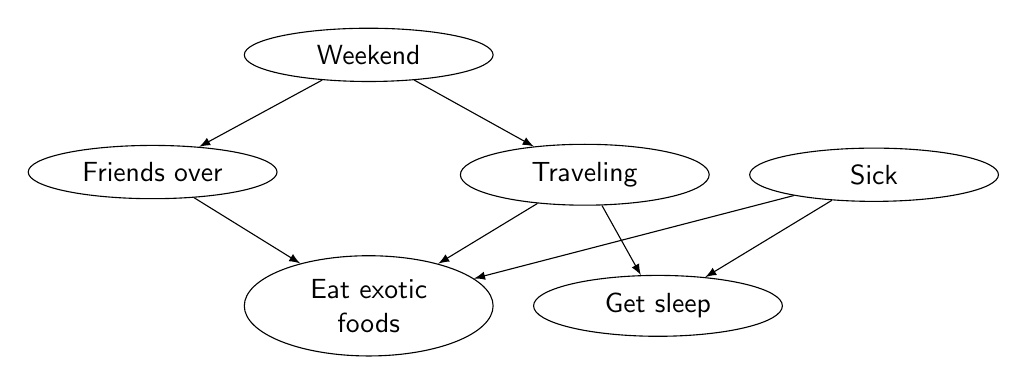
\begin{tikzpicture}[
  node distance=1cm and .5cm,
  bn/.style={draw,ellipse,text width=2cm,align=center}
    ]
    \node[bn] (w) {\attr{Weekend}};
    \node[bn,below right=of w] (t) {\attr{Traveling}};
    \node[bn,right=of t] (s) {\attr{Sick}};
    \node[bn,below left=of w] (f) {\attr{Friends over}};
    \node[bn,below right=of f] (eef) {\attr{Eat exotic foods}};
    \node[bn,right=of eef] (gs) {\attr{Get sleep}};
    \path (w) edge[-latex] (t)
    (w) edge[-latex] (f)
    (f) edge[-latex] (eef)
    (t) edge[-latex] (eef)
    (t) edge[-latex] (gs)
    (s) edge[-latex] (gs)
    (s) edge[-latex] (eef);
    \end{tikzpicture}
\end{center}

The random variables are:

\begin{itemize}
\item \attr{Weekend}: Is it the weekend?
\item \attr{Friends over}: Does the person have friends over?
\item \attr{Traveling}: Is the person traveling?
\item \attr{Sick}: Is the person sick?
\item \attr{Eat exotic foods}: Is the person eating exotic foods?
\item \attr{Get Sleep}: Is the person getting sleep?
\end{itemize}

\medskip

For the following questions, $A \perp B$ means that events A and B are
independent and $A \perp B | C$ means that events A and B are independent
conditioned on C.

\textbf{Use the concept of d-separation} to answer the
questions and show your work (i.e., state what the blocking path(s) is/are and what nodes block the path; or explain why each path is not blocked).

\textit{Example Question:} Is $\attr{Friends over} \perp \attr{Traveling}$? If NO, give intuition for why.

\textit{Example Answer:} NO. The path from Friends over -- Weekend -- Traveling is not blocked following the d-separation rules. Thus, the two are not independent. Intuitively, this makes sense as if say we knew that the person was traveling, it would make it more likely to be the weekend. This would then make it more likely for the person to have friends over.

\textbf{Actual Questions:}

\begin{enumerate}
\item Is $\attr{Sick} \perp \attr{Weekend}$?
  If NO, give intuition for why.


\item Is $\attr{Sick} \perp \attr{Friends over}\given \attr{Eat exotic
  foods}$? If NO, give intuition for why.


\item Is $\attr{Friends over} \perp \attr{Get Sleep}$? If NO, give
  intuition for why.

\item Is $\attr{Friends over} \perp \attr{Get Sleep} \given
  \attr{Traveling}$? If NO, give intuition for why.

\item Suppose the person stops traveling in ways that affect their
  sleep patterns (as various famous people have done).  Travel still
  affects whether they eat exotic foods.  Draw the modified network. (Feel free to reference the handout file for the commands for displaying the new network in \LaTeX).

\item For this modified network, is $\attr{Friends over} \perp
  \attr{Get Sleep}$? If NO, give an intuition why.  If YES,
  describe what observations (if any) would cause them to no longer be
  independent.

\end{enumerate}
\end{problem}


\section*{Solution}


\newpage
%%%%%%%%%%%%%%%%%%%%%%%%%%%%%%%%%%%%%%%%%%%%%
% Name and Calibration
%%%%%%%%%%%%%%%%%%%%%%%%%%%%%%%%%%%%%%%%%%%%%
\subsection*{Name}

\subsection*{Collaborators and Resources}
Whom did you work with, and did you use any resources beyond cs181-textbook and your notes?

\subsection*{Calibration}
Approximately how long did this homework take you to complete (in hours)? 

\end{document}
